\documentclass{beamer}

\usetheme{Hokie}
\usepackage{palatino}
\usepackage{amsmath}
\usepackage{tikz}
\def\checkmark{\tikz\fill[scale=0.4](0,.35) -- (.25,0) -- (1,.7) -- (.25,.15) -- cycle;} 

\title{Graph Algorithms for  Visualizing High Dimensional Data}
\author[Abhinav Shankaranarayanan Venkataraman]{Abhinav Shankaranarayanan Venkataraman \\{\small Directed by : Prof. Ricard Gavalda and Prof. Marta Arias}}
\institute{Universitat Politecnica de Catalunya (UPC), Barcelona}
\date{27 June 2016}

\graphicspath{{./}}
\DeclareGraphicsExtensions{.png}
\logo{
\includegraphics[height=0.5cm]{logo.png}}
\setbeamertemplate*{logo}
\newcommand{\HRule}{\rule{\linewidth}{0.5mm}} % Defines a new command for the horizontal
\begin{document}

\frame{\titlepage}

\section[Outline]{Outline}
\frame{
\tableofcontents
}

\section*{Project Details}
\frame{
\frametitle{Project Research Group}
\begin{itemize}
\item This project is carried out within the LARCA research group at UPC .
\item Researchers within LARCA have in the last two years began
collaborations with hospital and health agencies for the analysis of electronic
healthcare records [EHR].
\item In previous work within the group, they pro-
posed to organize the information in EHR in the form of graphs and hyper-
graphs, which can then be navigated by experts and mined with graph and
network theoretic tools.
\end{itemize}
}

\section{Introduction}
\subsection[What is a Community?]{Community Structure}
\frame{
\frametitle{What is Community?}
				\begin{figure}
	\centering
	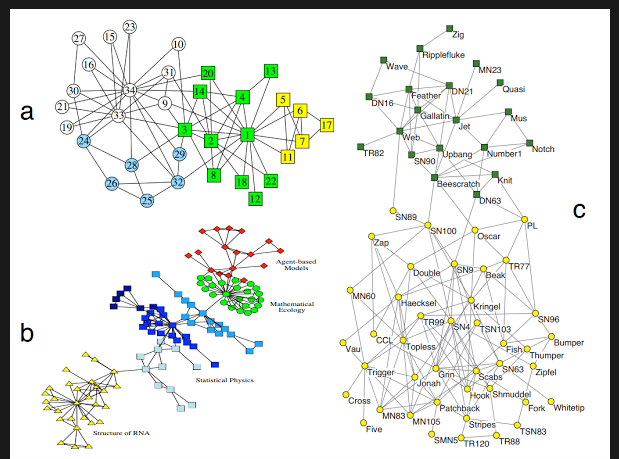
\includegraphics[scale=0.3]{comm.png}
	\caption{Communities: \cite{communitypaper}}
	\label{fig:test_down_sampling}
	\end{figure}

}
\subsection*{Goals of the Project}
\frame
{
	\frametitle{Goal of the Project}
	\begin{enumerate}
\item To survey a few algorithms that aim in community finding keeping in mind that the input is from the medical domain. 
\item To choose an algorithms that benefit the purpose of organizing graphs from medical domain and for the purpose of visualization.
\item To implement the algorithms and test the efficiency of the algorithm using variety of graphs.
\item To build a Graphic User Interface (GUI) which enables visualization of the raw input on a web browser by drawing graphs.

\end{enumerate}
}
\subsection*{Planning And Budget}

\frame{
\frametitle{Planning and Budget}
\begin{enumerate}
\item Planning: 
\begin{itemize}
\item Required knowledge acquisition
\item Paper Analysis
\item Design and Implementation
\item Testing I
\item Testing II

\item Report Writing

\end{itemize} 
\item Economic budget:  Hardware  budget, Software Budget, Human Resource Budget \\
\item Sustainability: Economically sustainable, Socially sustainable, Environmentally sustainable\\
\end{enumerate}
}

\section{State-of-the-art in Community Detection}

\frame{
\frametitle{State-of-the-art in Community Detection}
Communities are a part of the graph that have fewer ties with the rest of the system. A community should be densely connected, well separated from the rest of the network and the members of the network should be more similar among themselves than with the rest.
	\begin{figure}
	\centering
	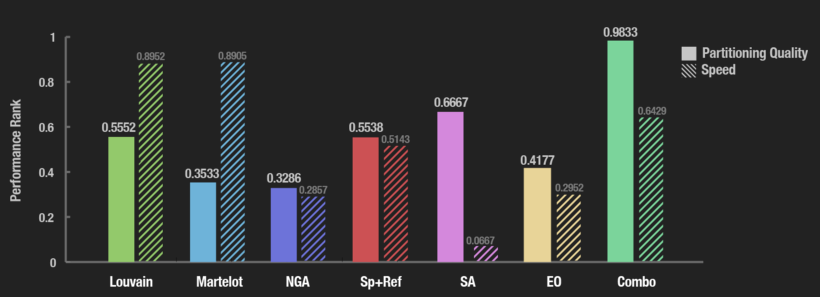
\includegraphics[scale=0.3]{lou.png}
	\caption{Exploring state of the art: \cite{generalcommunity}}
	\label{fig:test_down_sampling}
	\end{figure}
		
}
\section{Louvain Community Detection Algorithm}

\subsection{Louvain Method} \frame{
\frametitle{Louvain Algorithm \cite{communitypaper}}
Louvain algorithms is the state of the art community detection Algorithm. Louvain algorithm attempts to maximize modularity.
This algorithm has two phases. The diagram shows the 
\\

\begin{figure}[H]
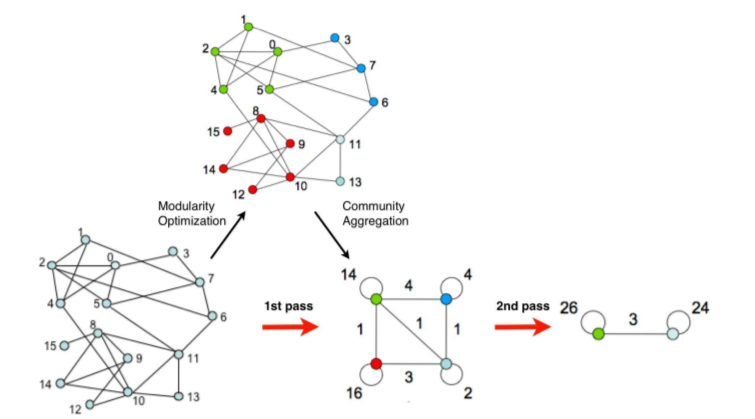
\includegraphics[scale=0.3]{loustep.png}
\caption{\label{loupic} Visualization of the steps of our algorithm.  This was taken from the paper "Fast unfolding of communities in large networks" \cite{Louvain}}
\centering
\end{figure}
}

\frame{
\frametitle{Louvain Algorithm Pseudocode}
Louvain Algorithm Pseudocode:
\begin{enumerate}
\item Repeat until local optimum is reached:
\begin{enumerate}
\item Phase1 : Split or partition the graph by optimizing modularity greedily
\item Phase2 : Agglomerate the found clusters into new nodes
\end{enumerate}
\end{enumerate}
}
\subsubsection[Phase1]{Louvain Method} 
\frame{
\frametitle{First phase in Louvain}
Louvain Algorithm Pseudocode for Phase1:
\begin{enumerate}
\item Assign a different community to each node.
\item For each node $v_i$
\begin{itemize}
\item For each $v_j$ $\in$ N($v_i$),consider removing $v_i$ from community of $v_i$ and place it in the community of $v_j$
\item Choose $v_i$ into community of neighbour that
leads to highest modularity gain (Greedy Choice).
\end{itemize}
\item Repeat until no improvement can be done
\end{enumerate}
}

\subsubsection[Phase2]{Louvain Method} 
\frame{
\frametitle{Second phase in Louvain}
Louvain Algorithm Pseudocode for Phase2:
\begin{enumerate}
\item Let each community $C_i$ form a new node $v_i$
\item  Let the edges between new nodes $v_i$ and $v_j$ be the sum of edges
between nodes in $C_i$ and $C_j$ in the previous graph
\end{enumerate}

}

\subsubsection[Mode of implementation]{Mode of implementation} 
\frame{
\frametitle{Mode of implementation}
The implementation of the Algorithm is in Python. pyLouvain is code that is freely available although considering the task perfomed by the project it is tough to use pyLouvain directly. Hence modifications were made to pyLouvain and some part of the code was reused. 
\\
The input data structure was altered. The Input file is stored in a matrix and its transpose is used to get the node set. This is  used to for a edge dictionary. 
}

\subsubsection[Experiments]{Louvain Method} 
\frame{
\frametitle{N until 2000 and Q=0.4, Scale-Free distribution Experiments}

	\begin{figure}
	\centering
	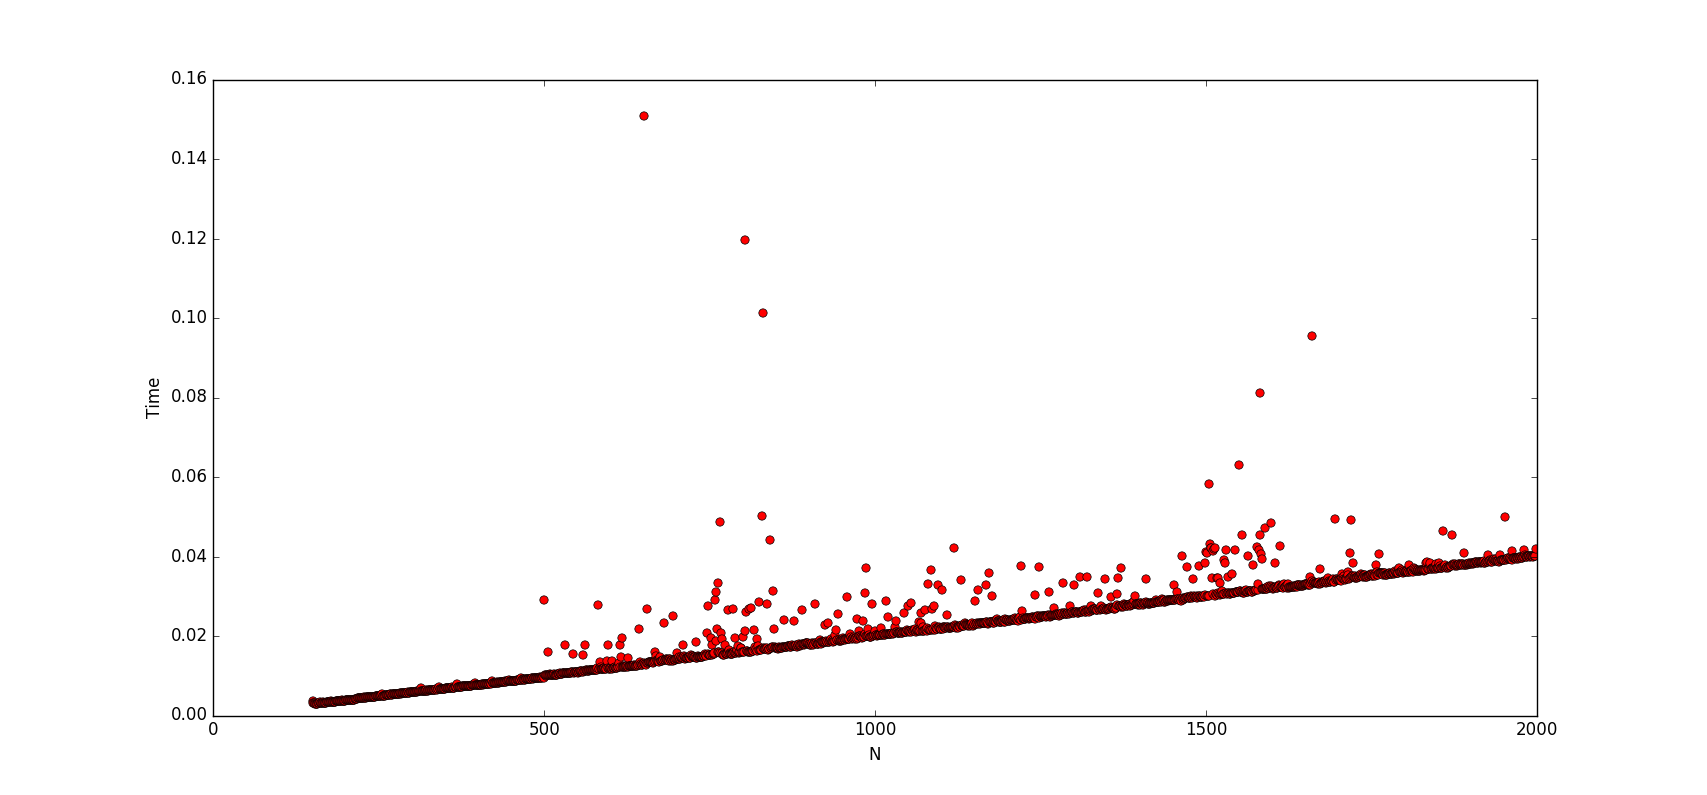
\includegraphics[scale=0.3]{e2000c.png}
	\end{figure}

}

\subsubsection[Experiments]{Louvain Method} 
\frame{
\frametitle{SNAP Experiments}

	\begin{figure}
	\centering
	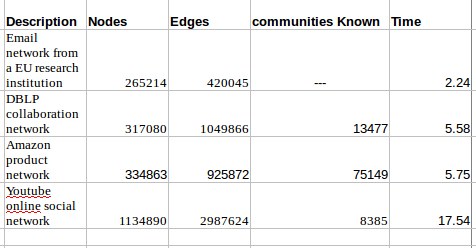
\includegraphics[scale=0.6]{snap.png}
	\end{figure}

}
\subsubsection[Experiments]{Louvain Method} 
\frame{
\frametitle{Famous Graphs Experiments}

	\begin{figure}
	\centering
	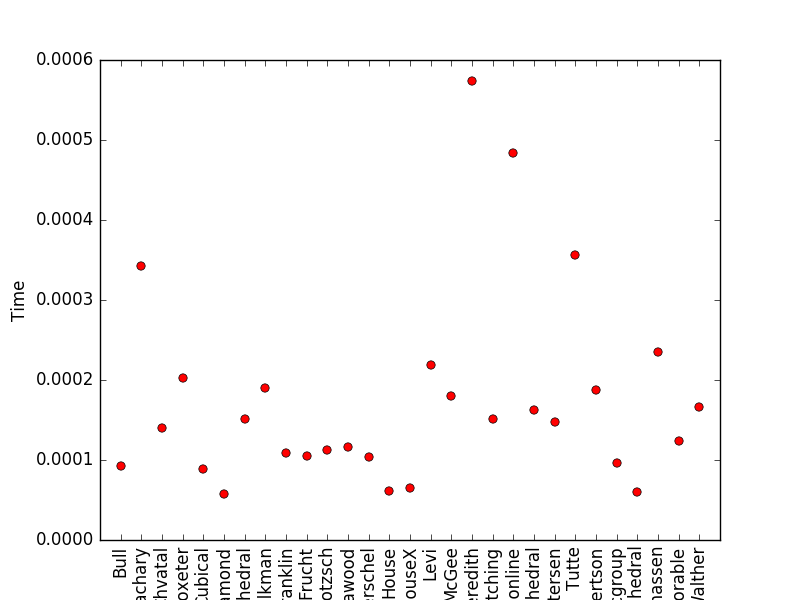
\includegraphics[scale=0.4]{fam.png}
	\end{figure}

}



\section{Visualization Libraries}
\frame{
\frametitle{Visualization  Libraries}
\begin{table}
	\centering
	\begin{tabular}{|c|c|c|c|c|} \hline \hline
	     & Protovis.js         & D3.js & Alchemy.js & Gephi      \\ \hline \hline
 JavaScript  & \checkmark   &\checkmark & \checkmark &  \\ \hline \hline
 JSON Object & \checkmark  &\checkmark &\checkmark & \\ \hline \hline
 Robust & &\checkmark & & \checkmark  \\ \hline \hline
Less Overhead & & &\checkmark &  \\ \hline \hline
	
	\end{tabular}
	\caption{Comparing Visualization methods}
	\label{tbl:kramer}
	\end{table}
}


\subsection{Alchemy.js}
\frame{
\begin{enumerate}
\item Alchemy needs three main units to form as an application namely: alchemy.css,
alchemy.js and data.
\item Five simple steps to connect the JSON object to draw the graph.
\item Tests:
\end{enumerate}

	\begin{figure}
	\centering
	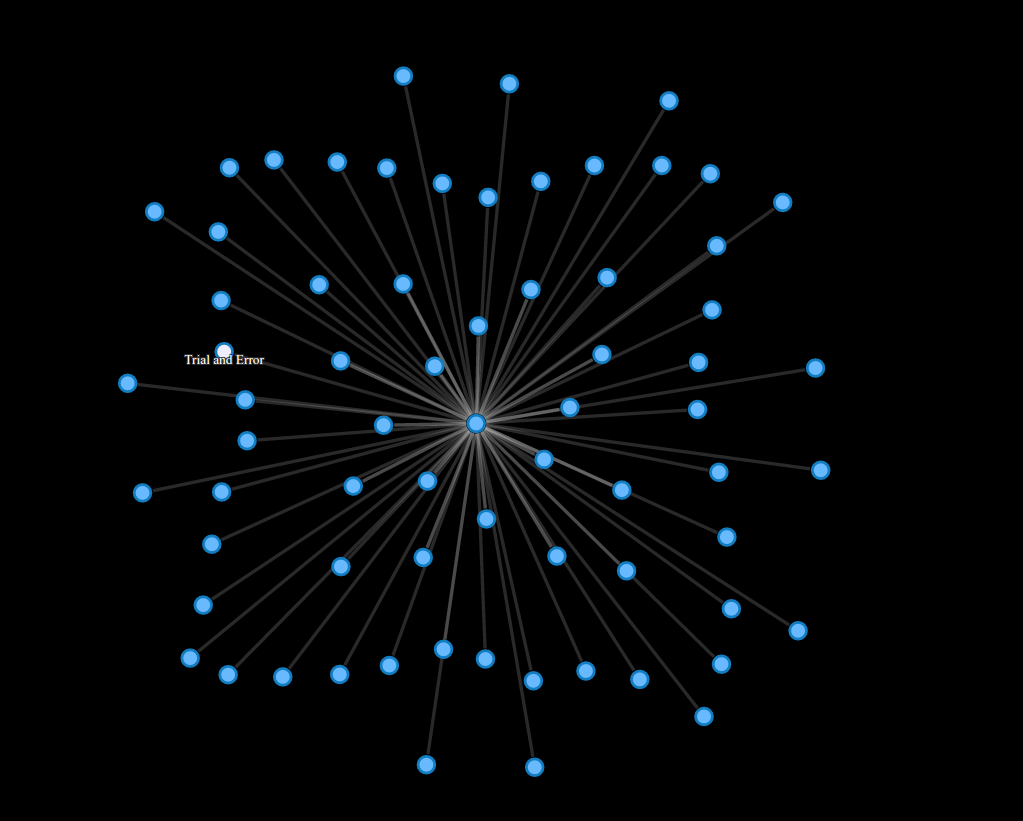
\includegraphics[scale=0.2]{t1.png}
	\end{figure}
}
\frame{
	\begin{figure}
	\centering
	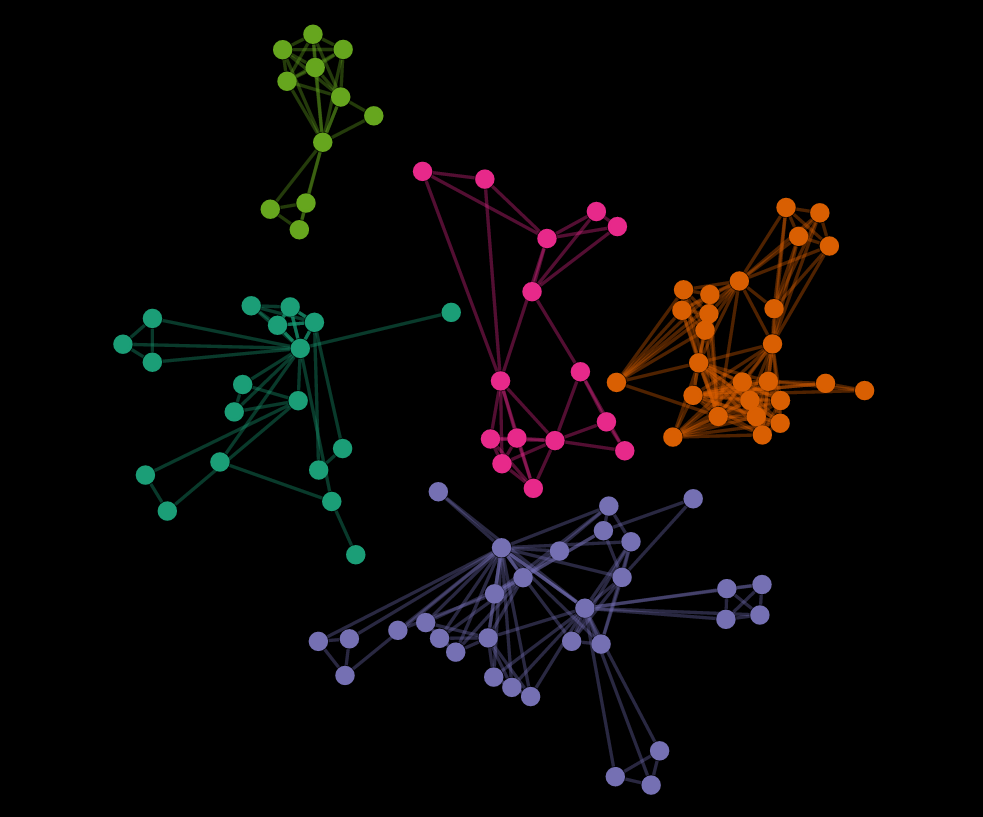
\includegraphics[scale=0.2]{t2.png}
	\end{figure}
}
\frame{
	\begin{figure}
	\centering
	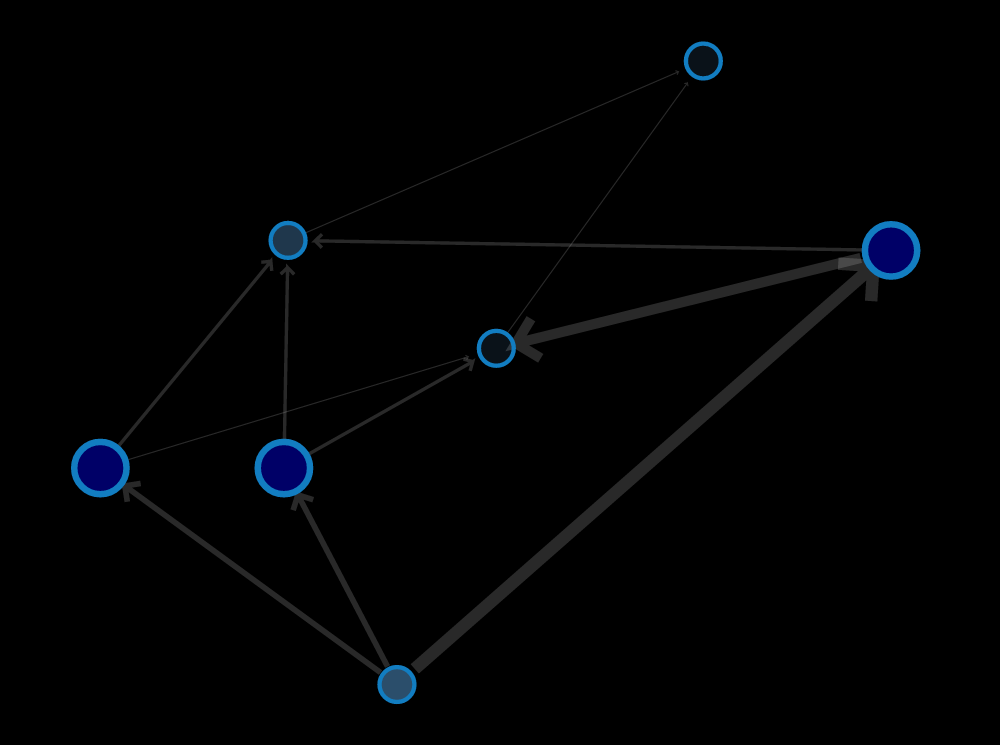
\includegraphics[scale=0.2]{t3.png}
	\end{figure}
}
\frame{
	\begin{figure}
	\centering
	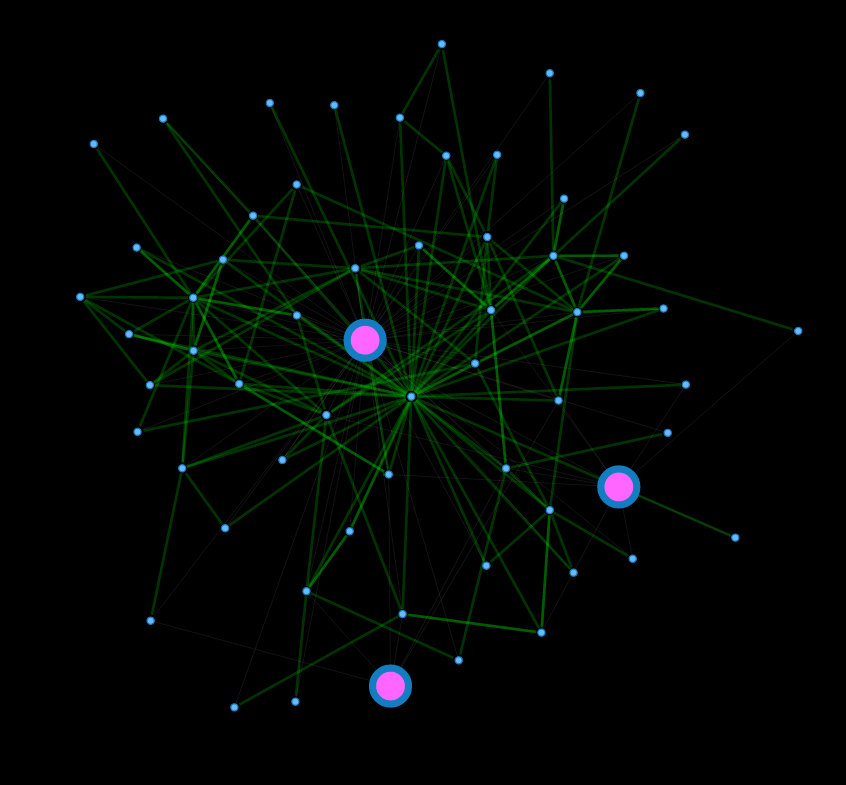
\includegraphics[scale=0.2]{t4.png}
	\end{figure}
}
\frame{
	\begin{figure}
	\centering
	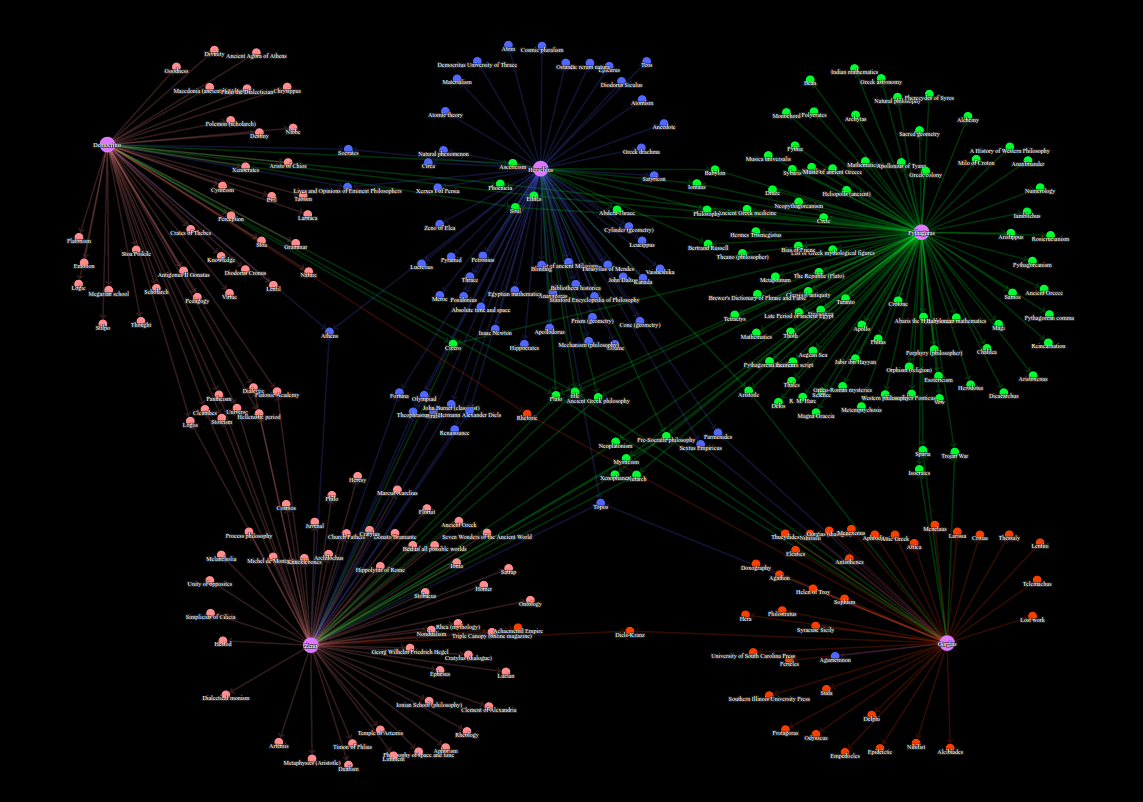
\includegraphics[scale=0.2]{t5.png}
	\end{figure}
}
\frame{
	\begin{figure}
	\centering
	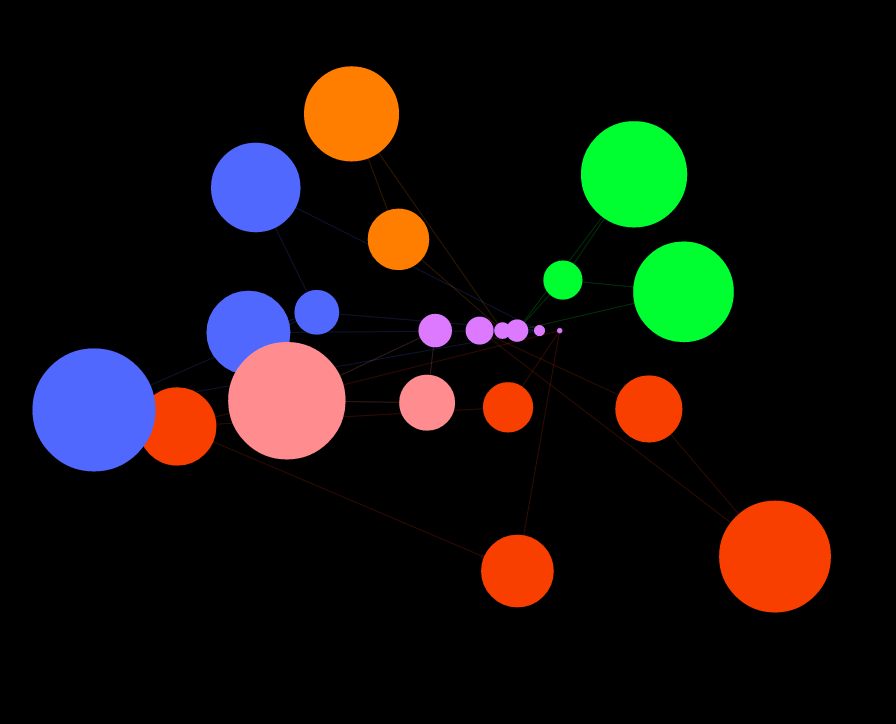
\includegraphics[scale=0.2]{t7.png}
	\end{figure}
}
\subsection[Experiments]{Alchemy.js} \frame{}
\subsection{Results} \frame{}

\section{Overall System}
\frame{
\frametitle{How it works?}
	\begin{figure}
	\centering
	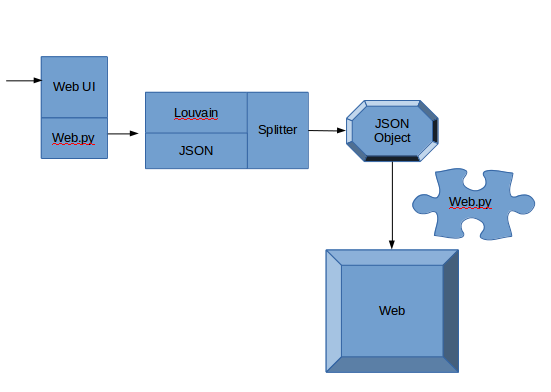
\includegraphics[scale=0.4]{arc.png}
	\end{figure}
}

\section{Conclusions}

\subsection{Personal Learning}
\frame
{
	\frametitle{Personal Learning}
The project gave a huge scope for exploring many softwares and trying out several of them. It gave an oppurtunity for me to learn Python to depth. My interest foe Data visualization and graph algorithms has increased. By trying a web application I got accustomed to using web frameworks and web technologies. 
Since the project had more scope for exploration.
My interest in Data Visualization has increased.
My interest in graphs has increased.
My python programming skill has also increased along with that I have also learned to code for web technologies on my own.
}

\subsection{Softwares and tool kits that were used}

\frame
{
	\frametitle{Software tools}
	\begin{enumerate}
		\item git
		\item github pages
		\item Linux OS
	\end{enumerate}
}



\section{References}

\frame
{
	\frametitle{List of References that were used}

\bibliographystyle{plain}
\bibliography{mybib}{}
}

\section{Gracies}
\frame
{
	\frametitle{Thank you}
Thank you for all those who supported me throughout the project.\\
It was a Great time at Barcelona working with Prof.Ricard and Prof.Marta.

}

\end{document}
